% !TEX root = ../VPJ.tex

\chapter{Schnittstellen}
\label{sec:Schnittstellen}

Schnittstellen

\section{Kommunikation zu Gewerk 2}


\label{sec:Gewerk2Protokoll}

Robotererrortypen beschreiben

\begin{table}[!ht]
	\centering
	\begin{tabular}{|r|c|l|}
		\hline
		Byte & Inhalt	&	Beschreibung \\
		\hline
			1  & Auftragsart & 1: Transport; 2: Parken; 3: Laden  \\
			2  & Position 1  & z.B. 11 \\
			3  & Position 2  & z.B. 32 \\
		  4  & AliveStatus & 1 senden nach Alive Anfrage \\
		  5  & *Reserved   &  \\
		\hline
	\end{tabular}
	\caption{Telegramm zu Gewerk 2}
	\label{tab:TelegrammZuG2}
\end{table}

%00: nichts; 01: unbekanntes Hindernis; 
%02: anderer Roboter; 03: direkt was gesehen?!? (flackert evtl)
%*1   X1: 1: Auf dem Weg; 2: Bin bei…; 
%X2 + X3 : Position 
%1: lebe ich noch? (Antwort senden) 0: ignorieren

\begin{table}[!ht]
	\centering
	\begin{tabular}{|r|c|l|}
		\hline
		Byte & Inhalt	&	Beschreibung \\
		\hline
			1  & Error &  Errortyp  \\
			2  & Akku  & Prozentwert als Integer \\
			3  & Hindernis & Hindernistyp \\
		  4  & *Reserved &  interner Roboterstatus \\
		  5  & AliveAbfrage  & 1: Roboterabfrage erfordert Antwort; 0: egal \\
		  6  & Status & $X_1X_2X_3$; 000: nichts zu tun \\
		  7  & Greifer   & 0:leer; 1:voll \\
		  8  & *Reserved &  \\
		  9  & *Reserved   &  \\
		\hline
	\end{tabular}
	\caption{Telegramm von Gewerk 2}
	\label{tab:TelegrammVonG2}
\end{table}

\begin{figure}[htb]
    \centering
    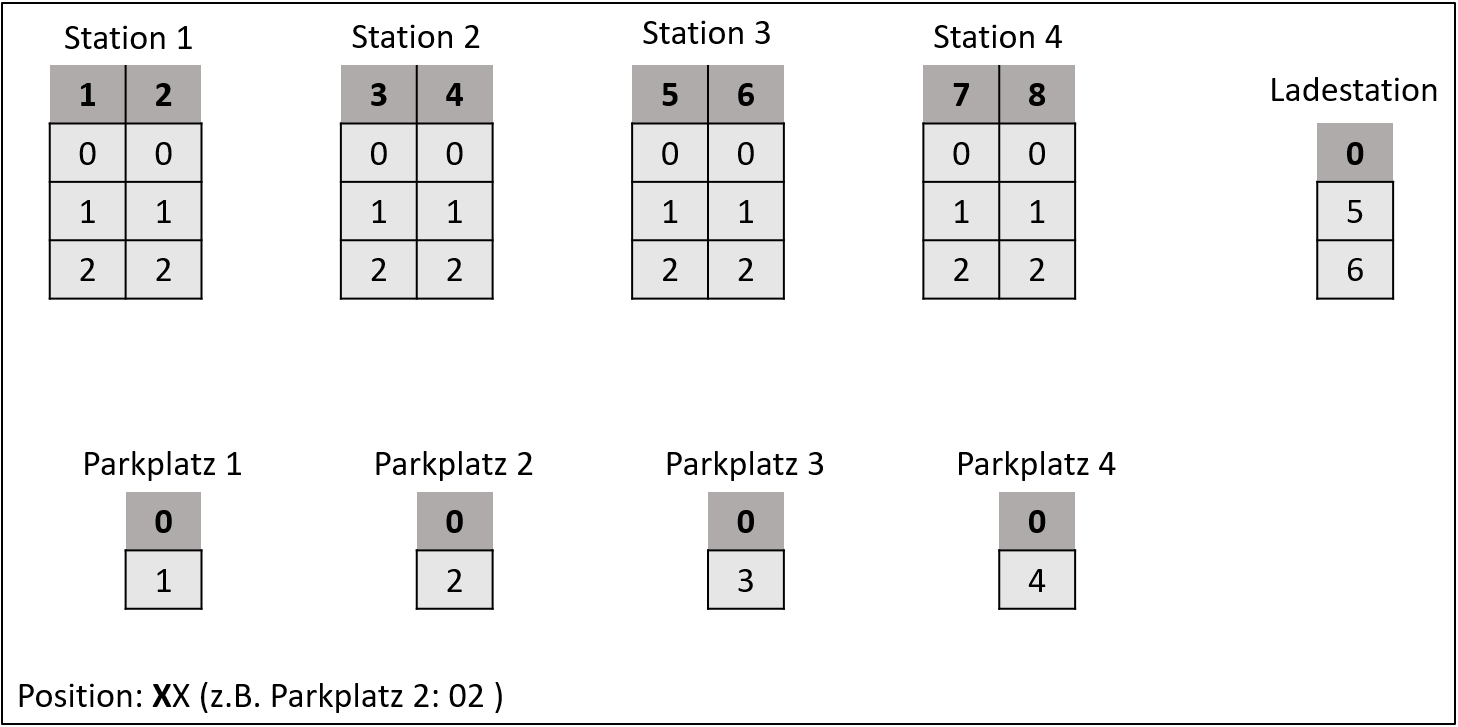
\includegraphics[width=0.9\textwidth]{Abbildungen/Positionskodierung.PNG}
    \caption{Positionskodierung}		
    \label{fig:Positionskodierung}
\end{figure}

Positionskodierung

\subsection{Sequenzdiagramm}
\label{sec:sequenzdiagram}

\begin{figure}[htb]
    \centering
    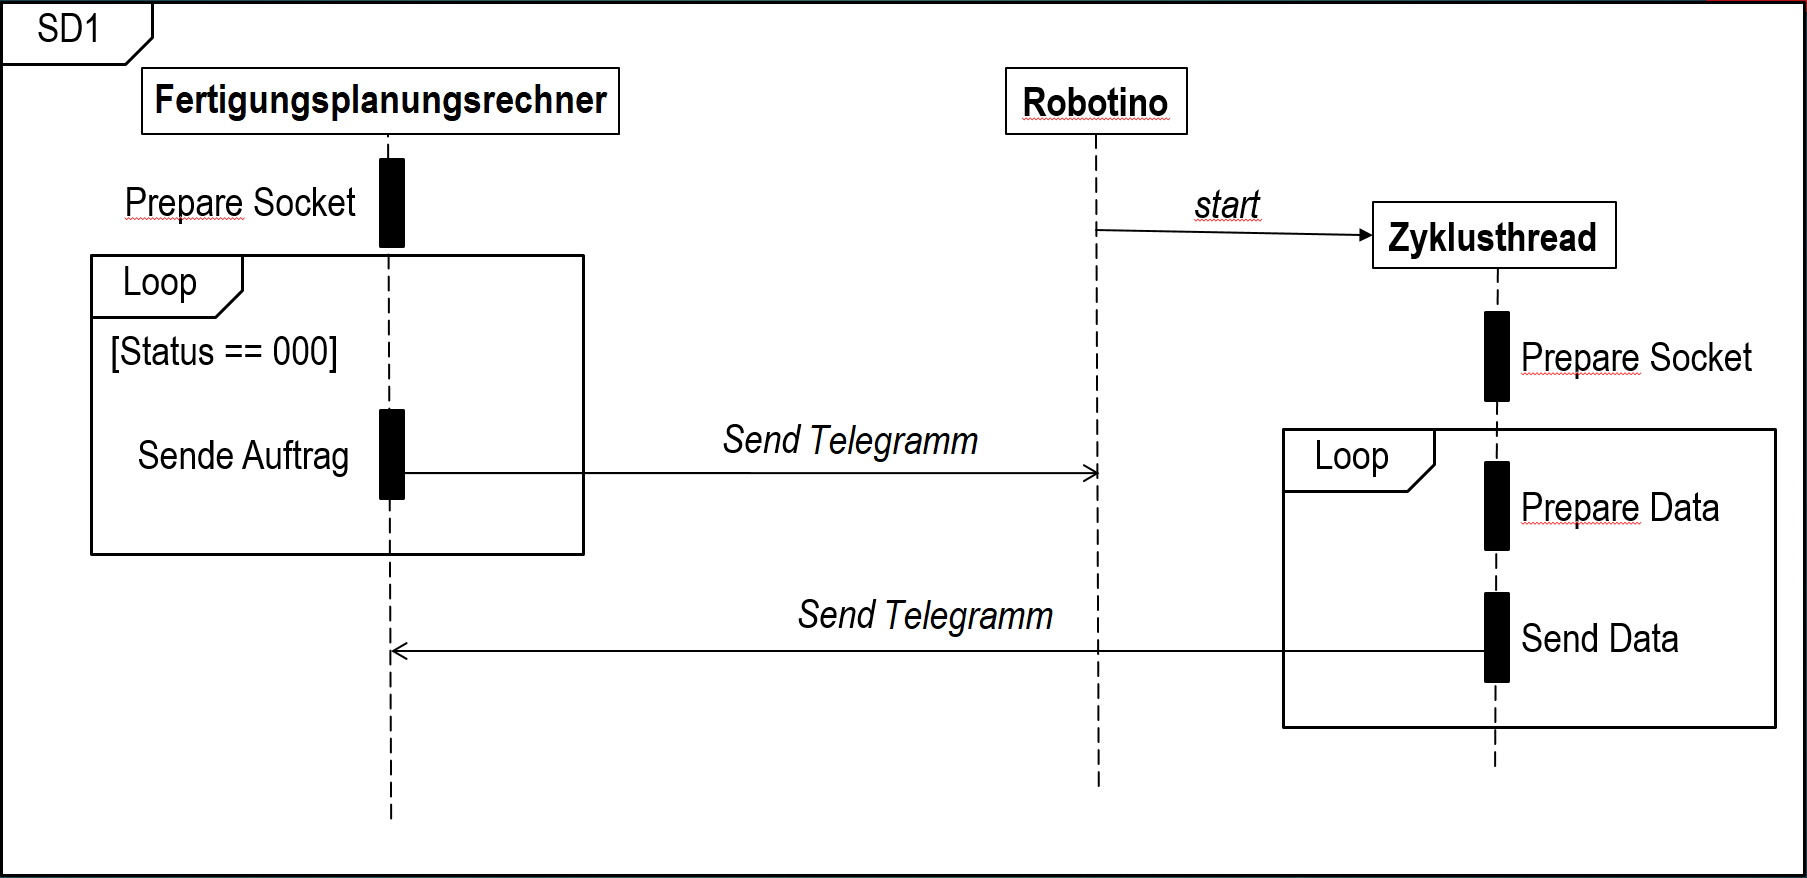
\includegraphics[width=0.9\textwidth]{Abbildungen/Sequenzdiagramm.PNG}
    \caption{Sequenzdiagramm}		
    \label{fig:Sequenzdiagramm}
\end{figure}

\inlinetodo{Sequenzdiagramm Kommunikation}
\inlinetodo{Telegram Gewerk 2}

\inlinetodo{Port vereinbarung}
\subsection{Fehlertypen und Behebung}
\label{sec:Error}

\subsubsection{Fehlertyp 1}
\subsubsection{Fehlertyp 2}
\subsubsection{Fehlertyp 3}
